\chapter{Discussion}
In this thesis, I presented the context-unified encoding (CUE) model.
To my knowledge, it is the first spiking neural network model of human memory that integrates activity-based short-term memory and weight-based long-term memory.
The same model matches a variety of behavioural data from serial and free recall experiments, but in contrast to previous models provides a hypothesis of a neural mechanistic explanation.

The CUE model exhibits many of the hallmark findings in memory research.
It shows the primacy and recency effect in immediate serial and free recall.
These effects get attenuated in delayed free recall, but in continuous distractor free recall the recency effect reappears.
Furthermore, the model was found to make very few transposition errors in serial recall, and if it does so nearby items are transposed.
In the free recall conditions, the model tends to start with items at the end of the list, recall nearby items together, and favour recall in forward direction.
Introducing delays and distractors attenuates these effects.
All of these observations match the findings from experiments with human subjects.

Not only are these qualitative effects reproduced, but also the quantitative match to the data is very good.
Only few significant differences, close to the number of differences expected by chance, were found.
One of these differences is worth considering in more detail: the model predicts a too strong forward bias in delayed free recall with both the lag \num{1} and \num{2} values of the CRP curve being significantly above the experimentally found values.
Interestingly, this is also highlighted as the least well matched aspect in the original TCM \parencite{Howard2002}.
While in that publication the TCM prediction is closer to the experimental data, the TCM prediction from a more recent paper \parencite{Sederberg2008} is closer to the CUE model prediction.
This makes it likely that the difference is not based on pure statistical chance, but that both the TCM and CUE model do not capture an essential aspect of memory, potentially related to the evolution of the context signal, that leads to reduced forward bias in delayed free recall.
It remains for future work, to precisely identify the reason for this mismatch and to extend the model.

Extending the CUE model with slow learning of either direct position to item associations or forward associations allowed the reproduction of the Hebb repetition effect qualitatively.
The involvement of such secondary learning should be considered a model prediction, as the effect could not be obtained without this extension.
Modelling the Hebb repetition effect also extends the model to effects across multiple trials of memory experiments.
This is done by only few memory models, in particular, neither the OSE, nor the TCM model attempted to match this kind of data.

As opposed to pure math models, the implementation as a spiking neural network allows the comparison and validation of the model against data from neural recordings in addition to the behavioural data.
In \cref{sec:aml-neural}, it was demonstrated that the proposed mechanism of association learning is able to explain neural data.
Unfortunately, neural data recorded from humans in memory experiments is still scarce, because invasive recordings can only be done when such recordings are required for medical reasons.
Nevertheless, implementing models with spiking neurons is worthwhile for several other reasons, despite the more complicated model construction and increased simulations times.
Drug effects, like scopolamine, can be more readily modelled, as was done with CUE model.
Also a higher degree of biological plausibility is achieved as one is forced to consider, for example, spiking noise and synaptic time constants.
This prevents common assumptions like arbitrary precision or perfectly orthogonal vectors made in many math models.

The spiking neural implementation also helps to constrain many parameter values.
Synaptic time constants, membrane time constants, and similar cellular physical quantities can be set to biologically plausible values reported in experimental findings.
These are fixed parameters that have not been adjusted for matching the behavioural data.
Similarly, as in the NEF, most connection weights are directly determined by least-squares minimization to implement a given function determined by the prescribed model architecture, hence the connection weights are fixed as well.
This leaves the model with very few free parameters.

To match the immediate serial recall, only two parameters were adjusted: the bias of the null choice $\minev$ and the input noise standard deviation $\recnoise$ in recall.
Both account for the fact that the recall network was restricted to recalling the items used within the memory experiment, while in reality a number of other items might interfere with the recall process.
For free recall experiments, one additional parameter $\psi$ is added that determines the probability of using the serial recall strategy even for free recall.
(For serial recall, a fixed values of $\psi = 1$ is implied as no free recall is allowed.)
Furthermore, in experiments with delay periods, a distractor rate $\drate$ needs to be set.
To simulate the effect of scopolamine the AML learning rate $\eta$ was adjusted.
However, in non-scopolamine conditions, it was treated as a fixed parameter and set to a value high enough to learn associations until the threshold for inhibition was achieved within the presentation duration.
Even higher values would not have any effect as long as it does not largely exceed the inverse of the synaptic time delay of the inhibition.
Lastly, only two additional parameters (weight decay rate and a separate learning rate) were introduced by the model extension to the Hebb repetition effect.

While few free parameters are desirable with respect to model parsimony, they should also be assigned similar values to model-related experimental conditions.
This is mostly the case for the CUE model.
The bias of the null choice in recall ranges from \numrange{0.03}{0.04} and values get monotonously smaller as the task difficulty increases with additional delays.
This corresponds to plausible longer recall attempts in more difficult experimental conditions.
Only a small difference is also observed in the distractor rates (\numrange{0.3}{0.4}) and the probability of using a serial recall strategy (zero for delayed recall and \num{0.1} in all other free recall conditions).
However, the noise standard deviation $\recnoise$ in recall differs by a factor of more than \num{1.5} without a clear relation to the experimental condition.
It is hard to hypothesize potential reasons for this difference as the parameter is accounting for things not explicitly modeled in recall.

It is also of interest how robust the model is against parameter changes.
I have not done a formal analysis of this because the model simulation times are prohibitive.
However, this also means that only a small set of parameter values without a lot of fine tuning has been tested (less than \num{200} combinations summed over all experimental conditions).
Given that finding the right parameters with few simulations is less likely if the model were highly sensitive to the parameter choice, a sufficient robustness to the exact choice of parameter values can be expected.

The CUE model is based on prior models of memory, but improves on them in important ways.
With regard to the OSE model, two main advancements can be stated.
First, the episodic memory buffer has been replaced with a much more plausible long-term memory mechanism that relies on synaptic-weight changes rather than reverberating neural activity.
Second, the CUE model also implements the mechanism providing the position tags fully in spiking neurons.

Implementing a long-term memory component based on the TCM in a spiking neural network provides a strong support for the biological plausibility of the TCM that previously was missing.
Certain simplifications of the TCM equations in this process to facilitate this implementation highlight which aspects of the TCM are essential and which do not contribute to the explanation of the data.
In particular, it also shows that certain assumptions, like perfectly orthogonal vectors, useful in the mathematical analysis, are not essential.
In addition, the modified TCM has been extended with a short-term memory component in the CUE model.
While the TCM has been posited as a single-store model, this has been criticized \parencite{Davelaar2008}.
The CUE model demonstrates that treating the TCM as part of a multi-store model is not unreasonable, provides good matches to the free recall data, and in addition allows matches to serial recall data.
Finally, the recall process in the TCM was not modeled in a particularly biologically plausible way and has been replaced with a more plausible spiking neural mechanism (\cref{sec:recall}).

In the broader context of memory models, the CUE model is unique as providing a low-level spiking network implementation, but matching high-level behavioural data.
This includes the recall process that is not explicitly modeled in many other models.
Furthermore, due to the item based context, there is no reinstantiation problem found in most context-based memory models.

A key part of the CUE model is the association matrix learning rule.
It provides insight into how one-shot learning without catastrophic forgetting is possible.
Several options and their biological plausibility of how this learning rule might be realized in the brain have been discussed in \cref{sec:aml}.
The main point there is that either some form of weight-sharing or symmetric decoder matrix is needed, or the input needs to be transformed into a sparse representation.
The dentate gyrus of the hippocampus exhibits such sparse firing and is implicated in associative learning, giving support to the latter hypothesis.
However, I also provided evidence that a symmetric decoder matrix might be learned in a biological plausible way.
Moreover, using the AML for learning simple pairwise associations, allows the reproduction of changes in firing rates that have been observed in recordings from human hippocampus.
These results are not only of interest for the CUE and TCM models, but many other cognitive models that assume the storage of associations in a similar association matrix without further explanation of how these associations are learned.

One potential criticism of the CUE model could target the method of position counting (\cref{sec:posnet}).
Only a limited number of positions can be represented, even though this number can be configured as large as permitted by neural resources.
If the number of positions is exceeded, the representation can be made to wrap around back to the first position.
Thus, the model does not need to fail catastrophically, but a specific pattern of recall errors could be introduced by encoding different sequences of items to the same positions.
However, an experimental test of such predictions will be hard, as long lists are likely required, and thus for most positions no item is recalled above chance.
It is worth highlighting that the position counting network in the CUE model can be replaced easily to test other hypotheses.
But it seems unlikely that the limited number of positions can be eliminated completely, because there will always be a limited number of almost orthogonal Semantic Pointers that fit into a vector space of given dimensionality.


%\begin{itemize}
    %\item firing rates!
    %\item basal ganglia involvement?
    %\item Control is the hard part
    %\item exact implementation of experimental protocol
    %\item fuzzy temp memory sensitive to noise and thus no alternative for context signal
%\end{itemize}


\section{Anatomical mapping}

Given that the CUE model is neural, it is of interest to consider how the parts of the model map to brain areas.
\Textcite{howard2005} proposed a mapping of the TCM model to brain areas that applies to a large degree also to the TCM-based part of the CUE model.
There are, however, some details to be reconsidered, and the OSE-based STM part of the model has not been discussed.

The medial temporal lobe (MTL) is known to be essential for free recall.
Damage to the MTL is detrimental to free recall performance \parencite{graf1984}.
Thus, we can assume that the TCM-related parts of the model reside in the MTL\@.

More precisely, the context storage network can be mapped  onto parahippocampal areas, in particular the entorhinal cortex (EC).
Its properties are consistent with the storage of non-spatial memories for tens of seconds.
In delay periods, stimulus dependent persistent activity can be observed \parencite{suzuki1997,young1997}.
\Textcite{quirk1992} showed EC has a higher mean firing rate than hippocampus, which is not caused by short bursts, and is thus compatible with the sustained maintenance of neural firing.
Also, the electrophysiological properties of the EC support integration \parencite{egorov2002}.
These findings are, however, based on intrinsic cell properties, whereas the CUE model uses recurrent connectivity for integration instead.
Note that the context network also contains integration ensembles that maintain the context signal over the timespan of seconds.

While the EC firing is modulated to some degree by the item position, this coding is more noisy than in the hippocampus \parencite{quirk1992}.
This indicates that EC codes for additional information.
\Textcite{frank2000} have shown that superficial EC employs retrospective coding, i.e., that it differentiates visits to the same position by the history leading up to that visit.
This is consistent with a context signal encoding the history of items leading up to the current item.

The other major components to map to brain structures are related to the learning and retrieval of associations in the $\mft$ and $\mtf$ matrices.
\Textcite{howard2005} stated that the $\mft$ matrix might not be implemented by a single anatomical region due to its complicated structure.
However, the updating equation for $\mft$ in the CUE model has been simplified, which makes the correspondence to a single region more plausible.
The learning of new associations in these matrices is attributed to the hippocampus by \textcite{howard2005}.
This is consistent with the results about the AML presented in \cref{sec:aml}.

The CUE model provides a more detailed description of the updating of the association matrices due to the neural implementation by means of the AML\@.
The learning network has recurrent connectivity to inhibit the learning once an association has been learned with the desired strength.
Recurrent connectivity is also found in the CA3 region of hippocampus.
Furthermore, CA3 receives input via the dentate gyrus and directly from entorhinal cortex, which could correspond to separate transmission pathways for the associated cue and target.
Interestingly, the AML highlighted the need to incorporate the decoder matrix $\mdec\Tr$ into the connections.
While I have shown it might be plausible that this connectivity is learned, the matrix could be reduced to the identity if the input ensemble were to provide orthogonalized inputs.
The dentate gyrus, providing input to CA3, is commonly assumed to perform such orthogonalization given its large neuron count, sparse firing, and neurogenesis \parencite[e.g.,][]{boss1987,jung1993-1,piatti2013}.
Thus, while the CUE model does not explicitly model the dentate gyrus (which is a significant research problem in itself), the learning rule used at least provides a principled reason for its existence.

Further evidence for this neuroanatomical mapping can be obtained from the connectivity between hippocampus and EC\@.
The superficial EC provides input to hippocampus, but does not receive direct input for hippocampus \parencite{witter2010}.
In contrast to that, the deep layers of EC receive input from hippocampus and might be relevant for recall, especially the recall of pre-experimental context.
This is consistent with the connectivity in the model where the context network projects to the association matrix learning network attributed to hippocampus.
The learning network for $\mft$ also projects back to an ensemble recalling the prior context before it gets combined in a different ensemble.

The short-term memory related components of the CUE model can be assumed to correspond to cortical areas, in particular the prefrontal cortex.
The prefrontal cortex has been found to be involved in working memory tasks in many studies \parencite[e.g.,][]{goldman-rakic1995,owen1997}


\section{Optimally fuzzy temporal memory}\label{sec:fuzzymem}
\Textcite{shankar2013} proposed a mathematical model of an optimally fuzzy temporal memory.
According to them it can replace the context signal in the TCM \parencite{howard2015}.
Thus it could also be relevant to the CUE model, but I argue below that a spiking neural version of this memory is unlikely to work without an implausible number of neurons.

The fuzzy temporal memory is constructed with the aim of representing past values of a function $f(t)$ with a scale-free fall off in accuracy.
Note that multiple such fuzzy temporal memories could be combined to represent a vector-valued function as needed for the context signal in the TCM or CUE models.
The memory itself consists of a set of independent, leaky accumulators given by the differential equation
\begin{equation}
    \od{c_i(t)}{t} = - s_i c_i(t) + f(t)
\end{equation}
where $s_i$ are decay constants.
This set of integrators is essentially computing a Laplace transform.
To readout the memory, the Laplace transform is inverted approximately with a linear operator $\mat L_k^{-1}$ given by
\begin{equation}
    \sbr{\mat L_k^{-1}}_{ij} = \frac{{(-1)}^k}{k!} s_i^{k+1} \sbr{\mat D_k}_{ij}
\end{equation}
where $\mat D_k$ is a square matrix that computes the $k$-th discrete derivative with respect to $s$.
The reconstructed $\hat{f}_t(t + t^*) = \sbr{\mat L_k^{-1} \vc c(t)}_i$ with $t^* = -k/s_i < 0$ estimates the values of $f$ at times $t + t_i^*$ in the past.
The reconstruction becomes more accurate as $k \rightarrow \infty$.

\Textcite{shankar2013} derive a signal to noise ratio, but use the magnitude of a delta impulse input to do so.
As the magnitude of a delta impulse is infinite in the limit, the signal to noise ratio also grows without bound for $k \rightarrow \infty$.
However, it is physically impossible to deliver a perfect delta impulse.
Instead it is more appropriate to analyze the steady state response for a fixed input $f(t) = u$.
In the context of the NEF, $u=1$ can be assumed without loss of generality because any change in the magnitude $u$ requires a matched change in the representational radius $\radius$ which will also scale the absolute error, keeping the relative error the same.
The steady state of the leaky integrators is then given by $c_i(t) = s_i^{-1}$.
This implies that NEF ensembles representing $c_i$ should use a radius of $\radius = s_i^{-1}$.

The amplification of the noise standard deviation is given by \textcite{shankar2013} as
\begin{equation}
    g_{\eta}(s_i, k) = \frac{\sqrt{2^k} s_i^{k+1}}{\delta_{s_i}^k k!}
\end{equation}
where $\delta_{s_i} = s_i - s_{i - 1}$. 
When following their proposal for optimal spacing of the $s_i$ by picking $t_i^* = (1 + \nu)^{i - 1} t_1^*$ for some constant $\nu > 0$, it follows that $\delta_{s_i} / s_i = \nu$ and the formula can be simplified to  % chktex 3
\begin{equation}
    g_{\eta}(s_i, k) = \frac{\sqrt{2^k} s_i}{\nu^k k!} = - \frac{\sqrt{2^k}}{\nu^k (k-1)! t_i^*} \text{.}
\end{equation}
Note that this amplification is not independent of $t_i^* = -k/s_i$, but increases as $t^* \rightarrow 0$.
This can be seen easily when adding some Gaussian noise to all $c_i$ before the reconstruction as done in \cref{fig:fuzzy-mem-noise-example}a.
It also refutes that ``the signal to noise ratio will remain constant over all timescales'' \parencite{shankar2013}; a statement based on the assumption of a perfect delta impulse.
However, as stated above, NEF ensembles should use a radius of $\radius = s_i^{-1}$ which scales the noise by the same factor and thus indeed leads to a constant amplification of the noise across timescales (\cref{fig:fuzzy-mem-noise-example}b) given by
\begin{equation}
    g_{\eta,\ped{NEF}}(\nu, k) = \frac{\sqrt{2^k}}{\nu^k k!} \text{.}
\end{equation}
\Cref{fig:fuzzy-mem-noise-ts}a shows this amplification for different parameter values.
When both $\nu$ and $k$ are chosen large enough, noise will actually be attenuated.
However, this also increases the timescale (\cref{fig:fuzzy-mem-noise-ts}b) and as such there is a trade-off between the time resolution of the memory and noise amplification.
This increase in timescale is given by
\begin{equation}
    \tau_i(\nu) = - {(1 + \nu)}^k t^*_i \label{eqn:fuzzymem-ts}
\end{equation}
and is caused by the discrete approximation of the derivative that relies on $t^*_{i - k}$ to $t^*_{i + k}$ for the reconstruction of $\hat{f}_t(t + t^*_i)$ and is dominated by $t^*_{i + k}$ (\cref{apdx:fuzzymem-derivative}).
\begin{figure}
    \centering
    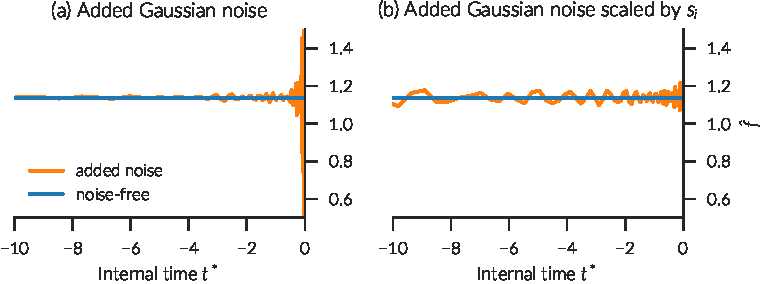
\includegraphics{figures/fuzzy-mem-noise-example}
    \caption[Example of the effect of noise on the fuzzy temporal memory.]{Examples of the effect of noise in the leaky integrators $c_i$ of the fuzzy temporal memory on the reconstruction $\hat{f}$. (a) Gaussian noise with mean zero and a constant standard deviation is added to the output of all integrators. (b) Gaussian noise with mean zero and standard deviation scaled by $s_i^{-1}$ is added to the output of all integrators.}\label{fig:fuzzy-mem-noise-example}
\end{figure}
\begin{figure}
    \centering
    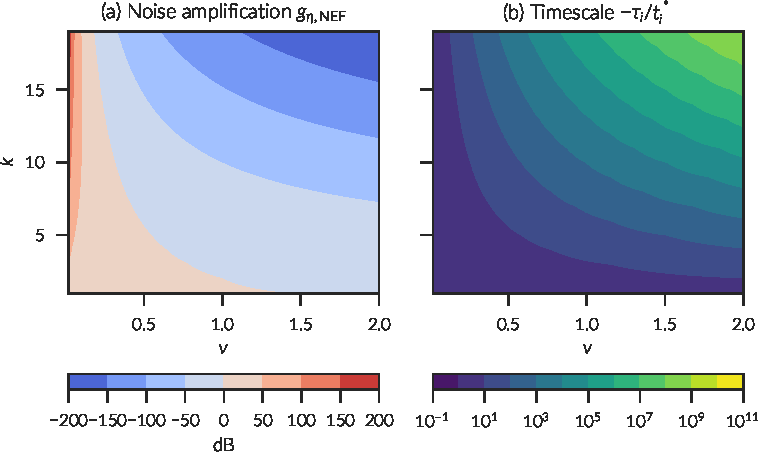
\includegraphics{figures/fuzzy-mem-noise-ts}
    \caption[Noise amplification and timescales in fuzzy temporal memory.]{(a) Noise amplification $g_{\eta,\ped{NEF}}$ in the fuzzy temporal memory. (b) Timescale $\tau_1$ for the $t^*_1$ reconstruction of the fuzzy temporal memory.}\label{fig:fuzzy-mem-noise-ts}
\end{figure}

Based on these equations, the total number of neurons $N_{\ped{tot}}$ required can be estimated as (\cref{apdx:fuzzymem-neurons})
\begin{align}
    N_{\ped{tot}}(t^*_1, k) &= N \dims\, g_{\eta,\ped{NEF}}^2(\nu, k) \del{M + 2k} \label{eqn:fuzzy-n-neurons}\\
    M &\geq \frac{\log(t^*_{\max} / t^*_1)}{\log(1 + \nu)} \\
    \nu &\leq \sqrt[k]{-\tau_1 / t^*_1} - 1
\end{align}
where $N$ is the number of neurons to represent a single dimension with sufficient accuracy (before the effect of the noise amplification), $\dims$ is the dimensionality of the input signal, $M$ gives the number of required leaky integrators, $\tau_1$ gives the desired smallest timescale, and $t^*_{\max}$ gives the desired timespan of the fuzzy memory.
Assuming that the fuzzy temporal memory is to be used for the TCM context signal, $\tau_1 \leq \SI{1}{\second}$ and $t^*_{\max} \geq \SI{10}{\second}$ are reasonable choices because ten item lists with a presentation rate one item per second are typical for the memory experiments matched in this work.
Furthermore, $N = 50$ and $\dims = 64$ can be used as conservative estimates.
Using \num{50}~neurons with maximum firing rates between \SIrange{200}{400}{\second^{-1}} is sufficient to read out the represented value, but not very precisely.
This default range of firing rates is much higher than firing rates typically observed in vivo.
Thus, the actual required number of neurons can be expected to be higher.
A dimensionality of $\dims = 64$ is also on the lower end to be able to fit sufficiently many almost orthogonal vectors into the space.
The CUE model uses four times as much, $\dims = 256$, dimensions.
Ultimately, the choice of $N$ and $\dims$ has only a minor influence on the results as they are just linear factors while the required number of neurons grows exponentially for $t^*_1,\ k \rightarrow \infty$.
The results for this choice of parameter values is shown in \cref{fig:fuzzy-mem-n-neurons}.
For most parameter combinations, the number of about $\num{13e6}$ neurons in the entorhinal cortex \parencite{west1998}, assumed to be the locus of the CUE/TCM context signal, and even the number of about \num{86e9} neurons in the human brain \parencite{azevedo2009} is far exceeded.
For an implementation with a realistic limit on the neuron number, $t^*_1$, but also $k$, needs to be sufficiently small.
\begin{figure}
    \centering
    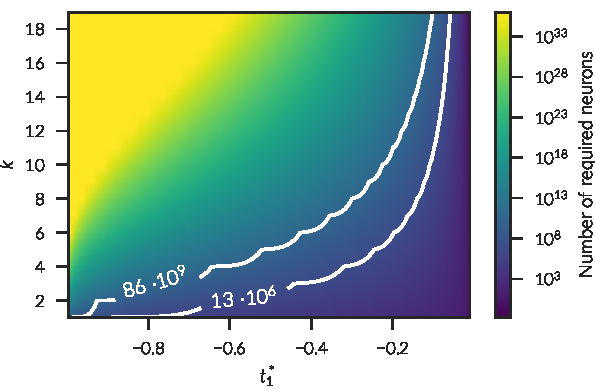
\includegraphics{figures/fuzzy-mem-n-neurons}
    \caption[Number of neurons required to implement a fuzzy temporal memory.]{Number of neurons required to implement a fuzzy temporal memory with a lower timescale of $\tau_1 = \SI{1}{\second}$ and a timespan of $t^*_{\max} = \SI{10}{\second}$. The white contours give the approximate number of neurons in the human entorhinal cortex (\num{13e6}) and human brain (\num{86e9}). See text for further details.}\label{fig:fuzzy-mem-n-neurons}
\end{figure}

Unfortunately, choosing small $t^*_1$ and $k$ is also problematic.
The error of the approximate inversion of the Laplace transform with Post's formula converges only at a rate of $1/k$ \parencite{vukimtuan2000}.
\Textcite{shankar2013} also comment themselves that $t^*_1$ needs to be kept sufficiently far from zero as it introduces a relative error in the order of $\bO\big(k^3\nu^2/96 t^{*2}_1\big)$ in the construction of the activity of $c_i$.

In conclusion, the fuzzy temporal memory has only a small parameter space that allows an implementation with feasible neural resources due to noise sensitivity.
This parameters space suffers from large relative errors unrelated to noise in the approximation of the inverse Laplace transform and discretized derivative.
Currently, it is not clear whether these non-noise related errors are sufficiently small to allow the fuzzy temporal memory to be used as a context signal in the CUE model.
At the same time it would require an increased number of neurons compared to the current implementation as each dimensions requires a set of leaky integrators, i.e.\ additional values have to be stored for each dimensions.
In comparison, the context network for \num{256}~dimensional vectors uses only \num{51225} neurons, and even when adjusting by a factor of \num{10}, this is many fewer neurons than found in the entorhinal cortex.


\section{Advances in large-scale cognitive modeling}
The primary objectives of building the CUE model lead to a number of advances in large-scale cognitive modeling that are worth summarizing, even though not all have been presented as part of this thesis.
Most importantly, optimizations for high-dimensional representations in neural networks (\cref{sec:hdrep};\ \cite{gosmann216}).
These allow the use of fewer neurons in such models, which ultimately allows more complex networks to be built without prohibitively long simulation times.
A similar benefit is the improved product network \parencite{gosmann2015-1}, as the calculation of products is often required, for example for the implementation of circular convolution.
Also a significant improvement to simulation times was achieved by the implementation of an optimization procedure in the Nengo simulator \parencite{gosmann2017}.
\Cref{sec:spa} described a new method for binding Semantic Pointers, the vector-derived transformation binding.
Even though it has not been used in the CUE model yet, it might provide a more precise binding and unbinding.
Finally, the independent accumulator network described in \cref{sec:ia} might not only be useful in recall, but for other large-scale models requiring clear decisions as part of a cognitive process.
